\clearpage
\section{Cell-based variables}
\label{sec:cell-based}

%%%%%%%%%%%%%%%%%%%%%%%%%
%                       %
%  Sequential Periodic  %
%                       %
%%%%%%%%%%%%%%%%%%%%%%%%%
\subsection{Sequential Periodic}

\subsubsection{Numeration}

%-------------%
%             %
% Cell 1.1.1. %
%             %
%-------------%
\begin{figure}[h]
  \centering
  \setlength{\unitlength}{1mm}
  \begin{picture}(105,60)(0,0)
    \thickbox{105}{60}
    \put( 1,0){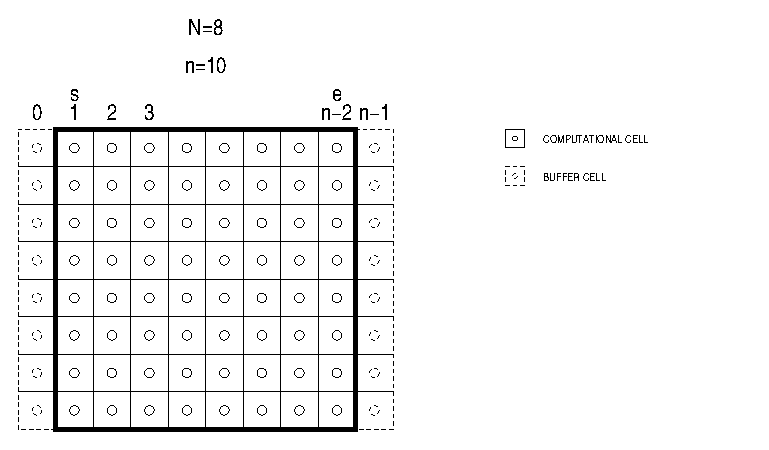
\includegraphics[scale=0.85]{Figures/Cell/1periodic_1sequential_1numeration.eps}}
  \end{picture}
  \caption{Numeration of sequential cell-based variable with periodic boundary 
           condition.}
  \label{cell:111}
\end{figure}
%
Description of Fig.~\ref{cell:111}:
%
\begin{enumerate}
  \item Program internally extends the resolution it by two: {\sf n=N+2}, to
        hold the information in the buffer/boundary cells.
  \item Computational cells are in the range {\sf 1} -- {\sf n-2}, which is 
        conveniently denoted by {\sf s} (start) and {\sf e} (end).
        Clearly, {\sf s=1} and {\sf e=n-2}, as indicated in the picture. 
\end{enumerate}

\subsubsection{Communication}

%-------------%
%             %
% Cell 1.1.2. %
%             %
%-------------%
\begin{figure}[h]
  \centering
  \setlength{\unitlength}{1mm}
  \begin{picture}(105,60)(0,0)
    \thickbox{105}{60}
    \put( 1,0){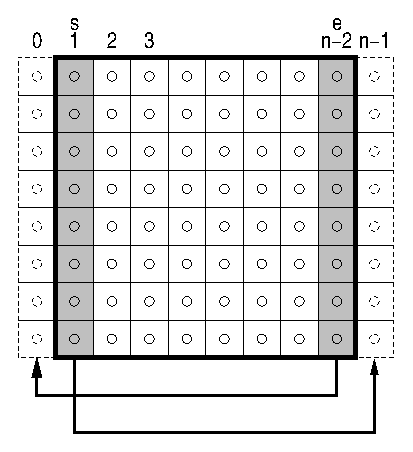
\includegraphics[scale=0.85]{Figures/Cell/1periodic_1sequential_2patterns.eps}}
  \end{picture}
  \caption{Communication patterns for sequential cell-based variable with 
           periodic boundary condition.}
  \label{cell:112}
\end{figure}
%
Description of Fig.~\ref{cell:112}:
%
\begin{enumerate}
  \item First computed column ({\sf s}) is sent to the end buffer~({\sf n-1}), 
        while the last computed column ({\sf e}) is sent to the start 
        buffer~({\sf 0}).
  \item The code from {\tt scalar\_exchange.cpp} to achieve this exchange is:
        \begin{verbatim}
         for_jk(j,k) {
           val[e_x+1][j][k] = val[s_x + o_x][j][k];
           val[s_x-1][j][k] = val[e_x - o_x][j][k];
         }
        \end{verbatim}
        Clearly, {\tt o\_x} (offset) is equal to {\bf zero} in this case.
\end{enumerate}

%%%%%%%%%%%%%%%%%%%%%%%
%                     %
%  Parallel Periodic  %
%                     %
%%%%%%%%%%%%%%%%%%%%%%%
\subsection{Parallel Periodic}

\subsubsection{Numeration}

%-------------%
%             %
% Cell 1.2.1. %
%             %
%-------------%
\begin{figure}[h]
  \centering
  \setlength{\unitlength}{1mm}
  \begin{picture}(105,135)(0,0)
    \thickbox{105}{135}
    \put( 1,0){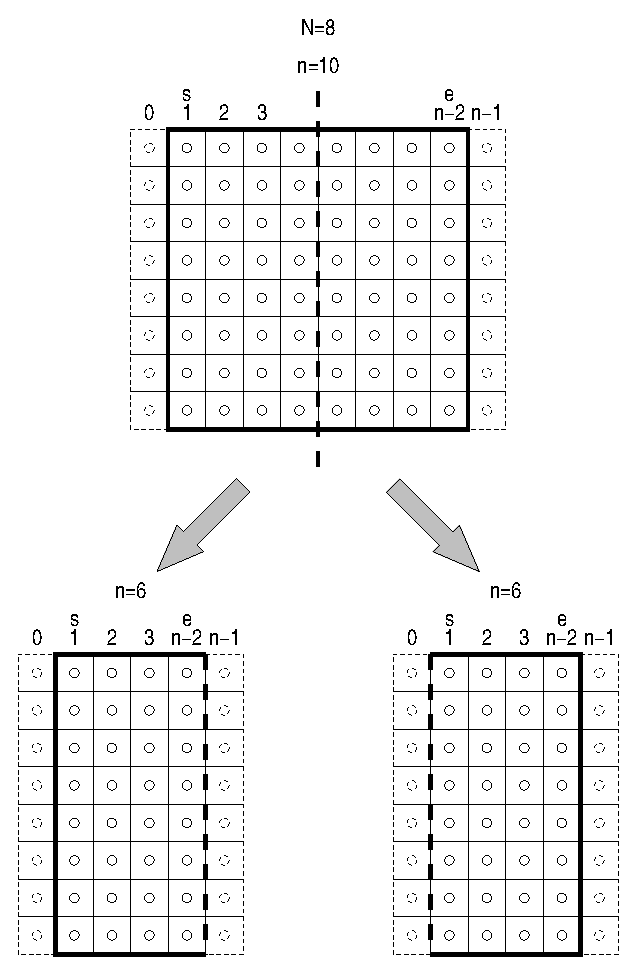
\includegraphics[scale=0.85]{Figures/Cell/1periodic_2parallel_1numeration.eps}}
  \end{picture}
  \caption{Numeration of cell-based variable with periodic boundary 
           condition for parallel computation.}
  \label{cell:121}
\end{figure}

Description of Fig.~\ref{cell:121}:
\begin{enumerate}
  \item In case of a parallel run, program divides the domain over processors.
        Meaning of {\sf n} changes in sense that it is no longer number of 
        cells defined by the user ({\sf N}) plus two, but number of cells 
        local to each processor, including buffers. 
  \item As for the sequential run with periodic boundary conditions, 
        computational cells are in the range 
        {\sf s} -- {\sf e} ({\sf 1} -- {\sf n-2}).
\end{enumerate}

\subsubsection{Communication}

%-------------%
%             %
% Cell 1.2.2. %
%             %
%-------------%
\begin{figure}[h]
  \centering
  \setlength{\unitlength}{1mm}
  \begin{picture}(105,75)(0,0)
    \thickbox{105}{75}
    \put( 1,0){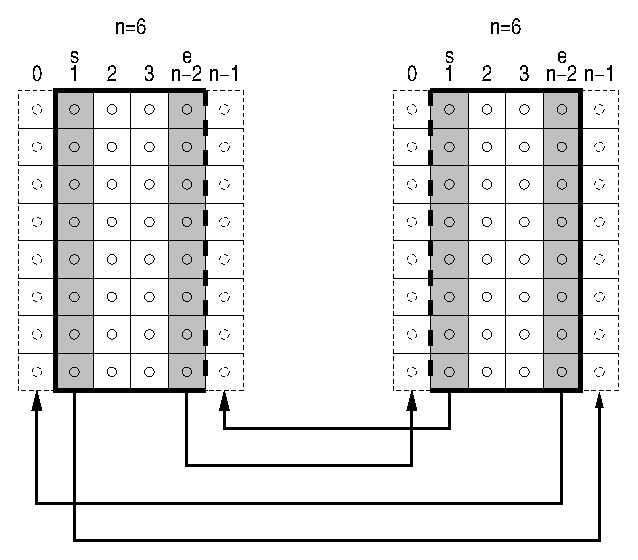
\includegraphics[scale=0.85]{Figures/Cell/1periodic_2parallel_2patterns.eps}}
  \end{picture}
  \caption{Communication patterns for parallel cell-based variable with 
           periodic boundary condition.}
  \label{cell:122}
\end{figure}

Description of Fig.~\ref{cell:122}:
\begin{enumerate}
  \item first computed column ({\sf s}) is sent to sending buffer at the start
        of the local domain~({\tt sbuff\_s}) and last computed column~({\sf e}) 
        is sent to sending buffer at the end of the domain~({\tt sbuff\_e}).
  \item The code from {\tt scalar\_exchange.cpp} to achieve this exchange is:
        \begin{verbatim}
        for_jk(j,k) {
          int l = k*nj()+j;
          sbuff_e[l] = val[e_x - o_x][j][k];   
          sbuff_s[l] = val[s_x + o_x][j][k];  
          rbuff_e[l] = val[e_x +  1 ][j][k];
          rbuff_s[l] = val[s_x -  1 ][j][k];
        }
        \end{verbatim}
        Clearly, {\tt o\_x} (offset) is equal to {\bf zero} in this case. The meaning
        of lines beginning with {\tt rbuff} is explained bellow.
  \item New buffer values will be received, after calls to MPI functions in 
        receive buffer at the start ({\tt rbuff\_s}) and the end ({\tt rbuff\_e})
        of the domain.   
  \item The received values are inserted into domain by:
        \begin{verbatim}
        for_jk(j,k) {
          int l = k*nj()+j;
          val[e_x+1][j][k] = rbuff_e[l]; 
          val[s_x-1][j][k] = rbuff_s[l];
        }
        \end{verbatim}
        This loop might re-write the values in boundary cells for parts of the
        domain not on the processor interface. To avoid it, the lines starting
        with {\tt rbuff\_s} in the loop under item~2.
\end{enumerate}

%%%%%%%%%%%%%%%%%%%%%%%%%%%%%
%                           %
%  Sequential Non-periodic  %
%                           %
%%%%%%%%%%%%%%%%%%%%%%%%%%%%%
\subsection{Sequential Non-periodic}

\subsubsection{Numeration}

%-------------%
%             %
% Cell 2.1.1. %
%             %
%-------------%
\begin{figure}[h]
  \centering
  \setlength{\unitlength}{1mm}
  \begin{picture}(105,60)(0,0)
    \thickbox{105}{60}
    \put( 1,0){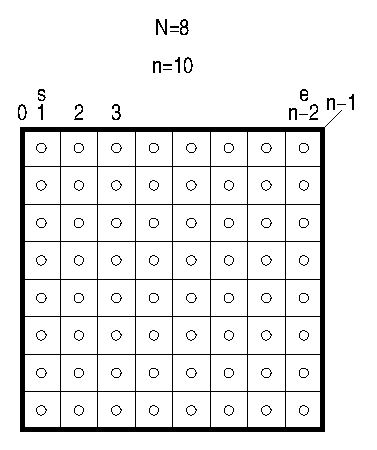
\includegraphics[scale=0.85]{Figures/Cell/2non-periodic_1sequential_1numeration.eps}}
  \end{picture}
  \caption{Numeration of sequential cell-based variable with non-periodic boundary
           condition.}
  \label{cell:211}
\end{figure}

Description of Fig.~\ref{cell:211}:
\begin{enumerate}
  \item Everything is the same as in Fig.~\ref{cell:111}, but boundary cells
        (column {\sf 0} and {\sf n-1}) coincide with the edge of the 
        computational domain. In other words, columns {\sf 0} and {\sf n-1}
        are not buffer, but boundary cells. 
\end{enumerate}

%%%%%%%%%%%%%%%%%%%%%%%%%%%
%                         %
%  Parallel Non-periodic  %
%                         %
%%%%%%%%%%%%%%%%%%%%%%%%%%%
\clearpage
\subsection{Parallel Non-periodic}

\subsubsection{Numeration}

%-------------%
%             %
% Cell 2.2.1. %
%             %
%-------------%
\begin{figure}[h]
  \centering
  \setlength{\unitlength}{1mm}
  \begin{picture}(105,135)(0,0)
    \thickbox{105}{135}
    \put( 1,0){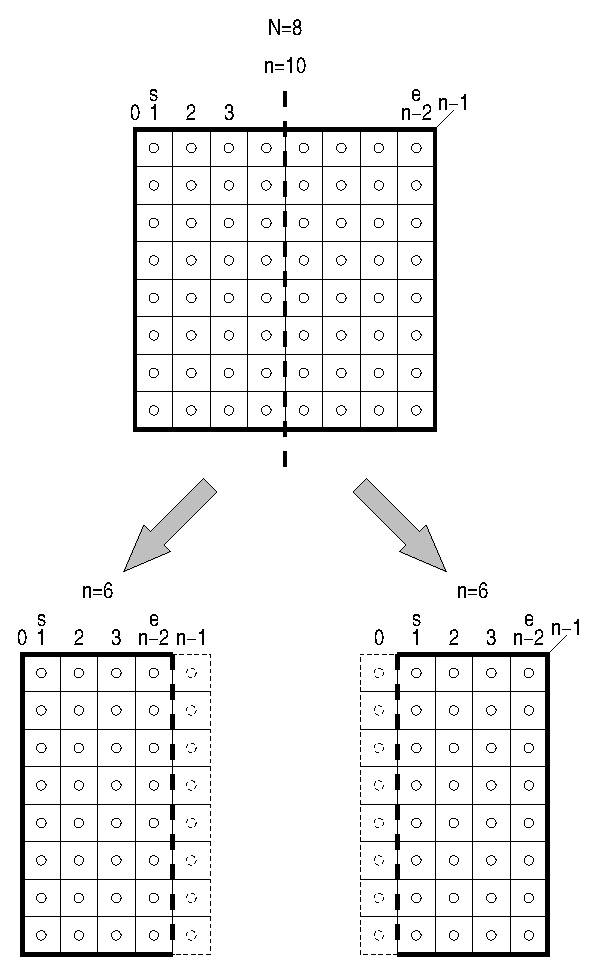
\includegraphics[scale=0.85]{Figures/Cell/2non-periodic_2parallel_1numeration.eps}}
  \end{picture}
  \caption{Numeration of sequential cell-based variable with non-periodic boundary
           condition.}
  \label{cell:221}
\end{figure}

Description of Fig.~\ref{cell:221}:
\begin{enumerate}
  \item Everything is the same as in Fig.~\ref{cell:121}, but boundary cells
        (column {\sf 0} in the left and column {\sf n-1} in the right domain) 
        coincide with the edge of the computational domain.
\end{enumerate}

\clearpage
\subsubsection{Communication}

%-------------%
%             %
% Cell 2.2.2. %
%             %
%-------------%
\begin{figure}[h]
  \centering
  \setlength{\unitlength}{1mm}
  \begin{picture}(105,60)(0,0)
    \thickbox{105}{60}
    \put( 1,0){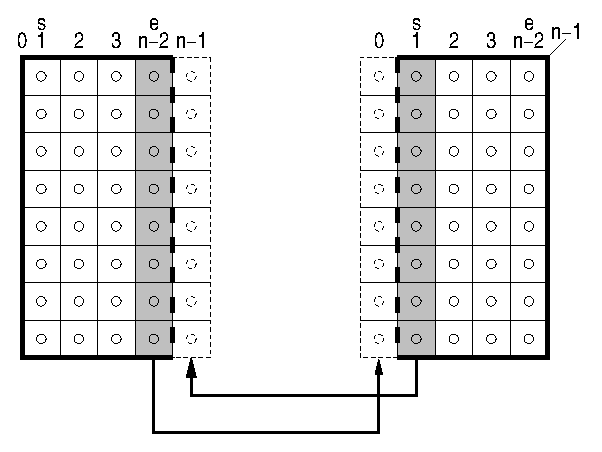
\includegraphics[scale=0.85]{Figures/Cell/2non-periodic_2parallel_2patterns.eps}}
  \end{picture}
  \caption{Communication patterns for parallel cell-based variable with 
           periodic boundary condition.}
  \label{cell:222}
\end{figure}

Description of Fig.~\ref{cell:222}:
\begin{enumerate}
  \item Everything is the same as in Fig.~\ref{cell:122}, but boundary cells
        (column {\sf 0} in the left and Clim {\sf n-1} in the right domain) 
        coincide with the edge of the computational domain.
\end{enumerate}

%------------------------------------------------------------------------notes-%
\vspace*{5mm} \fbox{ \begin{minipage}[c] {0.97\textwidth} %--------------notes-%
    {\sf Note on other coordinate directions} \\ %-----------------------notes-%

Since the grid for cell-based is non-staggered, the treatment in other 
coordinate directions is the same as the one explained here.

  \end{minipage} } %-----------------------------------------------------notes-%
%------------------------------------------------------------------------notes-%
